\section{Vectors and Scalars}

%\subsection{Force Vectors}

%I'm not sure we need a reference page for this - or maybe put it at the end?

\subsection{Scalars vs. Vectors}

\subsubsection{Vectors}

\blue{From TAM212 Reference Pages (Vectors and Bases):}

A \textit{vector} is an arrow with a length and a direction. Just like positions, vectors exist before we measure or describe them. Unlike positions, vectors can mean many different things, such as position vectors, velocities, etc. Vectors are not anchored to particular positions in space, so we can slide a vector around and locate it at any position.

\begin{figure*}[!h]
\centering
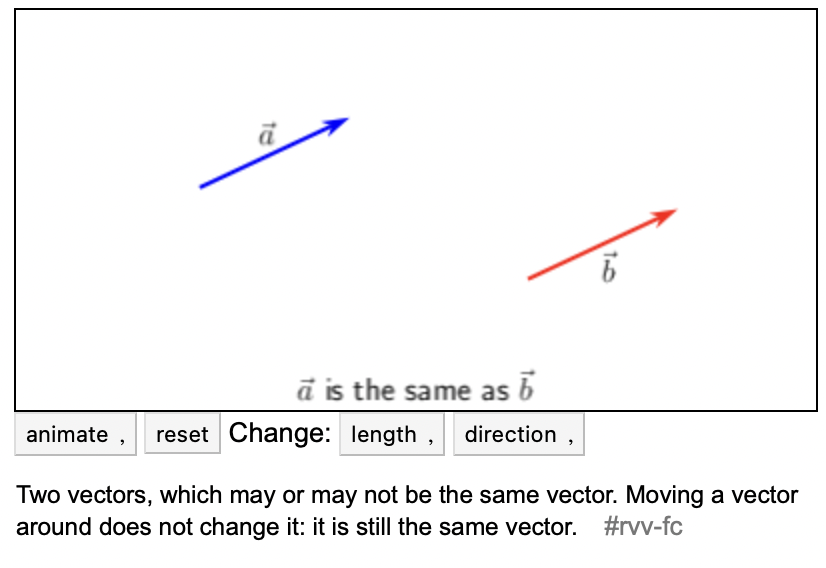
\includegraphics[angle=0, width=4in]{VectorsScalarsFigures/VectorDef.png}
\vspace{-2mm}
\caption{\small \blue{Taken from TAM212 Reference Pages (Vectors and Bases)}}
\vspace{-3mm}
\label{Fig:NewtonsLaws}
\end{figure*}

\subsubsection{Scalars}

While a vector represents magnitude and direction, a \textit{scalar} is a number that represents a magnitude, but with no directional information. Some examples of scalar quantities can be mass, length, time, speed, or temperature. 

\subsection{Vector Operations}

\subsubsection{Scaling Vectors}

\blue{Taken from TAM212 Reference Pages (Vectors and Bases)}

Vectors can be multiplied by a scalar number, which multiplies their length. 

\begin{figure*}[!h]
\centering
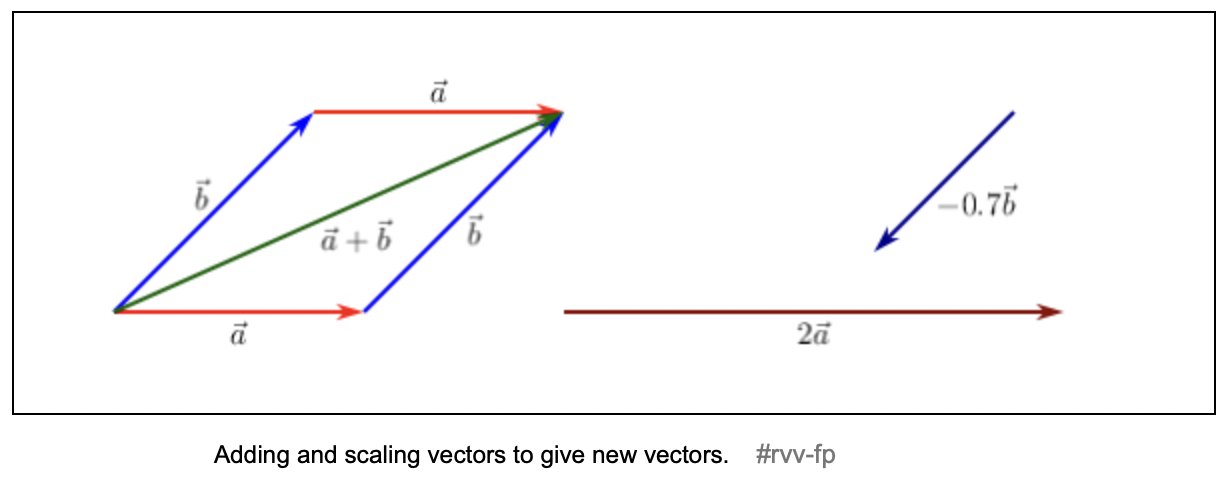
\includegraphics[angle=0, width=4in]{VectorsScalarsFigures/VecScaling.png}
\vspace{-2mm}
\caption{\small \blue{Taken from TAM212 Reference Pages (Vectors and Bases). Don't include the a+b vector - only keep one a and one b vector with their scaled counterparts.}}
\vspace{-3mm}
\label{Fig:NewtonsLaws}
\end{figure*}

\subsubsection{Vector Addition and Subtraction}

\blue{From TAM212 Reference Pages (Vectors and Bases):}

Vectors can be added or subtracted together, using the parallelogram law of addition or the head-to-tail rule.

\begin{figure*}[!h]
\centering
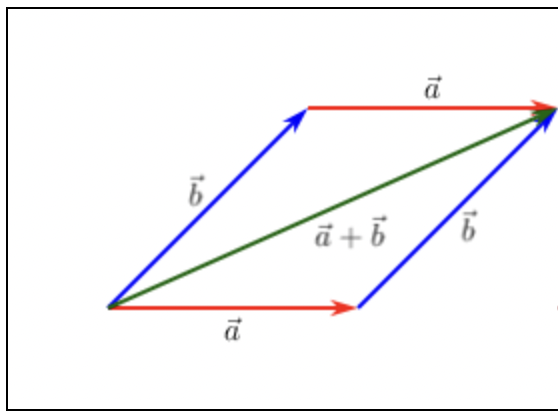
\includegraphics[angle=0, width=2in]{VectorsScalarsFigures/VecAddition.png}
\vspace{-2mm}
\caption{\small \blue{Taken from TAM212 Reference Pages (Vectors and Bases). Only include the left part of the figure, and add another part on the right that shows a-b.}}
\vspace{-3mm}
\label{Fig:NewtonsLaws}
\end{figure*}

\subsection{Unit Vectors}

\blue{Use the same content here as from the TAM212 Reference Pages (Vectors and Bases - Unit Vectors)}

\subsection{Vector Magnitude and Direction}

Vectors can be written as a magnitude (length) multiplied by the unit vector in the same direction as the original vector. 

\[\vec{A} = \|\vec{A}\|  \hat{u_A}\]

\blue{Insert the same content here as from the TAM212 Reference Pages (Vectors and Bases - Length of Vectors) for vector magnitude.}

The direction of a vector can be written as a unit vector by dividing the vector components by the vector magnitude. 

\begin{figure*}[!h]
\centering
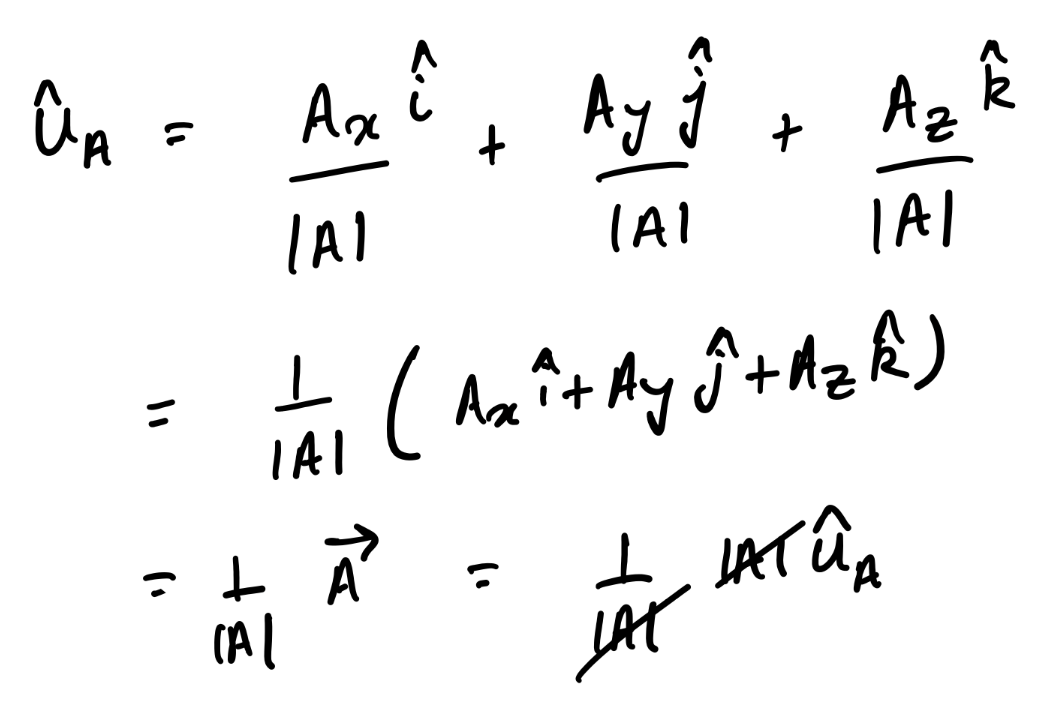
\includegraphics[angle=0, width=2in]{VectorsScalarsFigures/UnitVec.png}
\vspace{-2mm}
\caption{\small \blue{Taken from TAM210 Lecture Notes - Slide 3}}
\vspace{-3mm}
\label{Fig:NewtonsLaws}
\end{figure*}

Alternatively, the vector components can be determined geometrically via the angles of each component with respect to the Cartesian coordinates. 

\blue{Can probably make some sort of interactive figure here based on the image from TAM 210 lecture notes - slide 4}

\begin{figure*}[!h]
\centering
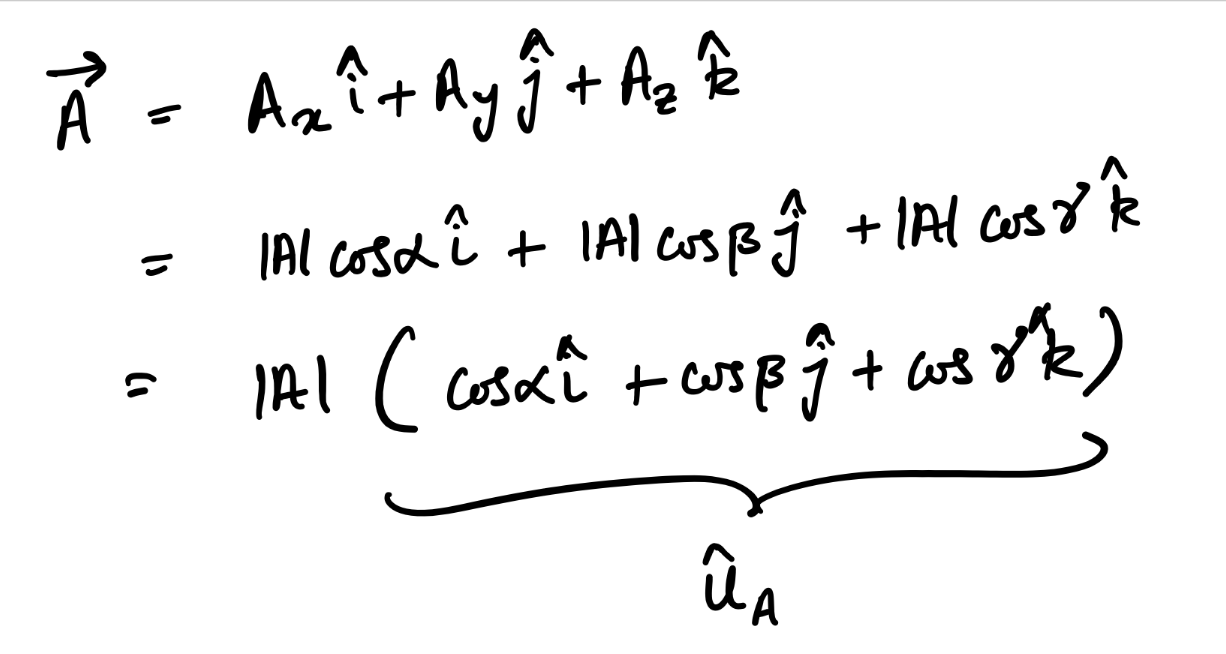
\includegraphics[angle=0, width=3in]{VectorsScalarsFigures/UnitVecAngles.png}
\vspace{-2mm}
\caption{\small \blue{Taken from TAM210 Lecture Notes - Slide 4}}
\vspace{-3mm}
\label{Fig:NewtonsLaws}
\end{figure*}


\subsection{Scalar and Vector Products}

\subsubsection{Dot Product}

\blue{Insert the same content here as from the TAM212 Reference Pages (Vectors and Bases - Dot Product).}

\subsubsection{\red{Cross Product}}

\red{Add something here about the three dimensional cross product?}

\blue{Insert the same content here as from the TAM212 Reference Pages (Vectors and Bases - Cross Product).}

\subsubsection{Vector Projection}

\blue{Insert the same content here as from the TAM212 Reference Pages (Vectors and Bases - Projection and Complementary Projection).}


